%%%%%%%%%%%%%%%%%%%%%%%%%%%%%%%%%%%%%%%%%
% Beamer Presentation
% LaTeX Template
% Version 1.0 (10/11/12)
%
% This template has been downloaded from:
% http://www.LaTeXTemplates.com
%
% License:
% CC BY-NC-SA 3.0 (http://creativecommons.org/licenses/by-nc-sa/3.0/)
%
%%%%%%%%%%%%%%%%%%%%%%%%%%%%%%%%%%%%%%%%%

%----------------------------------------------------------------------------------------
%	PACKAGES AND THEMES
%----------------------------------------------------------------------------------------

\documentclass{beamer}

\mode<presentation> {

% The Beamer class comes with a number of default slide themes
% which change the colors and layouts of slides. Below this is a list
% of all the themes, uncomment each in turn to see what they look like.

%\usetheme{default}
%\usetheme{AnnArbor}
%\usetheme{Antibes}
%\usetheme{Bergen}
%\usetheme{Berkeley}
%\usetheme{Berlin}
%\usetheme{Boadilla}
%\usetheme{CambridgeUS}
%\usetheme{Copenhagen}
%\usetheme{Darmstadt}
%\usetheme{Dresden}
%\usetheme{Frankfurt}
%\usetheme{Goettingen}
%\usetheme{Hannover}
%\usetheme{Ilmenau}
%\usetheme{JuanLesPins}
%\usetheme{Luebeck}
\usetheme{Madrid}
%\usetheme{Malmoe}
%\usetheme{Marburg}
%\usetheme{Montpellier}
%\usetheme{PaloAlto}
%\usetheme{Pittsburgh}
%\usetheme{Rochester}
%\usetheme{Singapore}
%\usetheme{Szeged}
%\usetheme{Warsaw}

% As well as themes, the Beamer class has a number of color themes
% for any slide theme. Uncomment each of these in turn to see how it
% changes the colors of your current slide theme.

%\usecolortheme{albatross}
%\usecolortheme{beaver}
%\usecolortheme{beetle}
%\usecolortheme{crane}
%\usecolortheme{dolphin}
%\usecolortheme{dove}
%\usecolortheme{fly}
%\usecolortheme{lily}
%\usecolortheme{orchid}
%\usecolortheme{rose}
%\usecolortheme{seagull}
%\usecolortheme{seahorse}
%\usecolortheme{whale}
%\usecolortheme{wolverine}

%\setbeamertemplate{footline} % To remove the footer line in all slides uncomment this line
%\setbeamertemplate{footline}[page number] % To replace the footer line in all slides with a simple slide count uncomment this line

%\setbeamertemplate{navigation symbols}{} % To remove the navigation symbols from the bottom of all slides uncomment this line
}
\usepackage{commath}
\usepackage{graphicx} % Allows including images
\usepackage{booktabs} % Allows the use of \toprule, \midrule and \bottomrule in tables

\graphicspath{ {images/} }

%----------------------------------------------------------------------------------------
%	TITLE PAGE
%----------------------------------------------------------------------------------------

\title[Randomnized Algorithm]{Randomnized Algorithm for Finding Min-Cut } % The short title appears at the bottom of every slide, the full title is only on the title page

\author{Renming Qi \and Vincent Chiu} % Your name

%\institute[UCLA] % Your institution as it will appear on the bottom of every slide, may be shorthand to save space
%{
%University of California \\ % Your institution for the title page
%\medskip
%\textit{john@smith.com} % Your email address
%}
\date{\today} % Date, can be changed to a custom date

\begin{document}

\begin{frame}
\titlepage % Print the title page as the first slide
\end{frame}


%----------------------------------------------------------------------------------------
%	PRESENTATION SLIDES
%----------------------------------------------------------------------------------------

%------------------------------------------------
\section{First Section} % Sections can be created in order to organize your presentation into discrete blocks, all sections and subsections are automatically printed in the table of contents as an overview of the talk
%------------------------------------------------

\subsection{Subsection Example} % A subsection can be created just before a set of slides with a common theme to further break down your presentation into chunks




\begin{frame}
\frametitle{Motivation}
\begin{itemize}
	\item Ford Fulkerson has a large running time for finding the minimum cut for large integer flows. It runs in pseudo polynomial time.  This is a big drawback.
	\item There exists a randomnized algorithm that could solve the minimum cut problem that is not affected by large integer flows.
\end{itemize}


\end{frame}


\begin{frame}
\frametitle{Randomnized Algorithms }
\begin{block}{Waiting for first Success}<1->
Bob has only p=10\% possibility to pass a math exam, but you can take the exam as many times as you like. 
\begin{itemize}
	\item What's possibility of taking the exam only once?
	\item How about 10 times, 100 times 
\end{itemize}
\end{block}
\begin{itemize}
	\item Using the following formula 
	\begin{equation*}
	\Pr\left(\text{Within N exams, Bob passes}\right)=1-(1-p)^N
	\end{equation*}
\end{itemize}
With N=5, P = 0.41. With N=10, P = 0.65.
With N=100, P = 0.99 \\
So after a large number of tries, Bob will finally pass the exam for almost sure even if he know nothing.

\end{frame}
%------------------------------------------------
\begin{frame}
\frametitle{Randomnized Algorithms}
\begin{block}{ what's randomnized algorithms}<1->
\begin{enumerate}
	\item Random decision
	\item Random result
\end{enumerate}
We have showed even if it can only succeed with small probability, we can get the right answer by running it many times. 	
\end{block}
\begin{block}{Why we need that}<2->
\begin{enumerate}
	\item Simpler
	\item New way to analysis complex system
\end{enumerate}
\end{block}
\end{frame}
\section{Analysis of Contract Algorithm}

%------------------------------------------------

\begin{frame}
%<<<<<<< HEAD
%\frametitle{The Problem}
%\begin{block}{Instance}
%An undirected graph G(V, E)	
%\end{block}
%\begin{block}{Question}
%
%Find the global minimum cut. Note that global here refers to the fact that any cut is allowed, as there is no sink or source in our graph for this type of problem.
%\end{block}
%		
%
%
%=======
\frametitle{Instance and Question}
\begin{itemize}
		\item Instance: An undirected graph G(V, E)
		\item Question: Find the global minimum cut. Note that global here refers to the fact that any cut is allowed, as there is no sink or source in our graph for this type of problem.
\end{itemize}
\end{frame}

\begin{frame}
\frametitle{What is minimum cut?}
\begin{itemize}
		\item The minimum cut is a natural measure of how robust the graph is. If you want to disconnect the graph into 2 components, it is the least number of edges you have to cut.
		\item Red line is a cut
		\item Green line is a min cut
\end{itemize}
\begin{center}
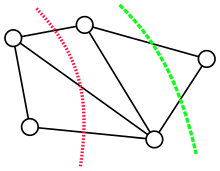
\includegraphics[width=0.5\textwidth]{min_cut_png_version}
\end{center}

%>>>>>>> 967e54436a283a31a74a877f0c3654de6739fcf6
\end{frame}
%\begin{frame}
%	The minimum cut is a natural measure of how robust the graph is. If you want to disconnect the graph into 2 components, it is the least number of edges you have to cut.
%	\begin{figure}
%		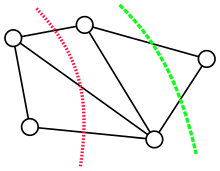
\includegraphics{images/220px-Min_cut_example.png}
%
%	\end{figure}
%	\end{frame}
%\begin{frame}
%\frametitle{The Problem }
%\begin{itemize}
%		\item The minimum cut is a natural measure of how robust the graph is. If you want to disconnect the graph into 2 components, it is the least number of edges you have to cut.
%\end{itemize}
%\end{frame}

\begin{frame}
\frametitle{Definitions for Understanding Contraction Algorithm}
\begin{itemize}
	\item David Karger: discovered the contraction algorithm in 1992.
	\item Multigraph: An undirected graph that is allowed to have multiple edges between the same pair of nodes.
	\item Supernode: consists of nodes that have been combined due to contracting edges
\end{itemize}
\end{frame}

\begin{frame}

\frametitle{What is contraction algorithm?}

\begin{itemize}
	\item Randomly choose edge e = (u,v) of G, we take this edge and we create a new graph G' where the nodes that edge e was connected to become one node. 
	\item Recursively call the contraction algorithm until only 2 nodes are left. 
	
\end{itemize}


\end{frame}


\begin{frame}
\frametitle{What is contraction algorithm? }


Successful run of the contraction algorithm on a graph with 10 nodes.  The minimum cut is of size 3, note the 3 edges between the white node and the red node at the rightmost diagram.
\begin{figure}
	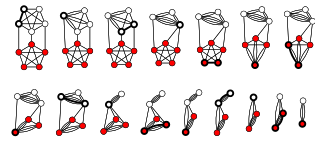
\includegraphics[scale=0.5]{kargers_diagram}
\end{figure}
An error case
\begin{figure}
	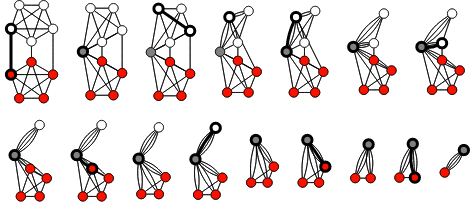
\includegraphics[scale=0.3]{images/error_case}
\end{figure}
\end{frame}




\subsection{Error Probability}
\begin{frame}
\frametitle{Analysis of Contract Algorithm}
\begin{overlayarea}{\linewidth}{\textheight}
\begin{onlyenv}<1-2,5>
\begin{block}{Success Rate of Contract Algorithm}
The Contraction Algorithm returns a global min-cut of G with probability at least $1/\binom n2$	
\end{block}
\end{onlyenv}

\begin{onlyenv}<2>

\begin{block}{Proof}

Let's assume the global min-cut in graph G(V,E) is (A,B) and it has size k. The set of cut edges is F
\begin{enumerate}[{Case}.1]
\item An edge in F is contracted. Then game over.
\item The contracted edge is not in F. We can continue contracting.
\end{enumerate}
So, how large or small is the possibility $p_1$ that we end our game at first step? \\
\end{block}
\end{onlyenv}
\begin{onlyenv}<3>
	\begin{figure}
		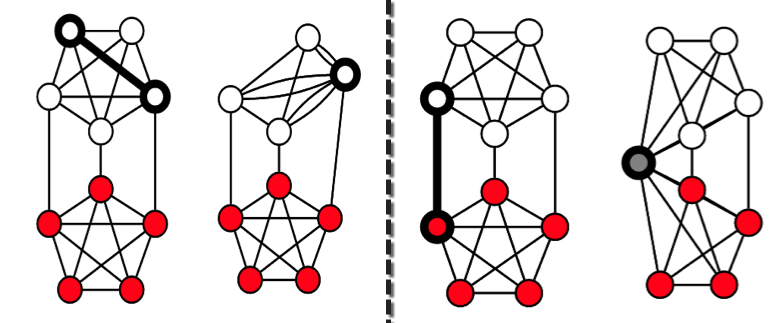
\includegraphics[scale=0.4]{images/contract}
	\end{figure}	
	\begin{enumerate}[{Case}.1]
\item An edge in F is contracted. Then game over.
\item The contracted edge is not in F. We can continue.
\end{enumerate}

\end{onlyenv}
\begin{onlyenv}<4>
\begin{block}{Proof Cont'd}<4>
When contracting the first edge randomly,
\begin{enumerate}
	\item $\forall v \in V, deg(v)\geq k$
	\item $\abs{E}\geq \frac{1}{2}nk$
	\item $p_1\leq \frac{k}{\frac{1}{2}nk}=\frac{2}{n}$
\end{enumerate}
After j iteration, there are n-j super-nodes in the current graph G'.
\begin{enumerate}			
	\item $\abs{E'}\geq \frac{1}{2}(n-j)k$
	\item $p_j\leq \frac{k}{\frac{1}{2}(n-j)k}=\frac{2}{n-j}$
\end{enumerate}
\begin{equation*}
\Pr\left(\text{Correct}\right)\geq \prod _{i=0}^{n-3}(1-p_n) = \prod _{i=0}^{n-3}{\Bigl (}1-{\frac {2}{n-i}}{\Bigr )}={\binom n2}^{-1}
\end{equation*}
\end{block}
\end{onlyenv}
\subsection{Time Complexity}	
\begin{onlyenv}<5>
\begin{block}{Time Complexity}
After contracting $n^2\log{}n$ times, the probability that we do not find the optimal solution
\begin{equation*}
p_e = (1-{\binom n2}^{-1})^{n^2\log{}n} \approx 1/n
\end{equation*}
so the running time is $\mathcal{O}(n^2\log{}n\times \abs{E})$
\end{block}

\end{onlyenv}

\end{overlayarea}

\end{frame}
%------------------------------------------------

%------------------------------------------------



\begin{frame}
\frametitle{References}
\footnotesize{
\begin{thebibliography}{99} % Beamer does not support BibTeX so references must be inserted manually as below
\bibitem[Kleinberg, 2006]{p714} Kleinberg and Tardos (2006)
\newblock Finding the Global Min Cut
\newblock \emph{Algorithm Design} 714 - 719



\bibitem[Karger Diagram]{p1} Thore Husfeldt  (2012)
\newblock Karger's Algorithm Diagram
\newblock \emph{Wikipedia} 

\bibitem[Min Cut Diagram]{p1} Kilom691 (2012)
\newblock Min Cut Diagram
\newblock \emph{Wikipedia} 


\end{thebibliography}
}
\end{frame}


%------------------------------------------------

\begin{frame}
\Huge{\centerline{The End}}
\end{frame}

%----------------------------------------------------------------------------------------

\end{document}